\section{Introduction}
\label{sec:bcoolintro}
This chapter presents \bcool, a dedicated (meta)language to capture the knowledge about system integration. With \bcool, an \emph{integrator} can deal with the complexity of the coordination of heterogeneous behavioral models by capturing coordination patterns at the language level (see Figure~\ref{fig:proposedworkflow}). Coordination patterns are captured into operators that specify how \dse of different language behavioral interfaces are combined and interact. Once specified in \bcool, integrators can shared such knowledge thus allowing reusing and tuning of coordination patterns. Also, \emph{system designers} can use the \bcool specification to generate an explicit coordination model when specific models are used. Such a formal coordination model enables system designer to perform verification and validation activities on the coordinated system.     
	
In this chapter, we illustrate the use of \bcool through a simple example: the coordination of the models of a coffee machine. To build the model, we base on two languages: a state-based language named Timed Finite State Machine (TFSM) and an action-based language named Activity. The model of the coffee machine is thus heterogeneous. We propose to coordinate these models by specifying a \bcool operator between these languages. We use this operator as running example all through the chapter. 

%\todo{This represents a typical case of separation of concern in which one domain is better described by a data-flow language and other is described by a control flow language}

We begin this chapter by presenting the running example; we show the languages with its behavioral interface. Then, we continue presenting the abstract syntax and the semantics of \bcool. Afterward, we present the implementation of \bcool into the GEMOC studio. To finish the chapter, we evaluate and compare our approach with coordination languages and frameworks and we conclude.


\begin{figure}
	\begin{center}
		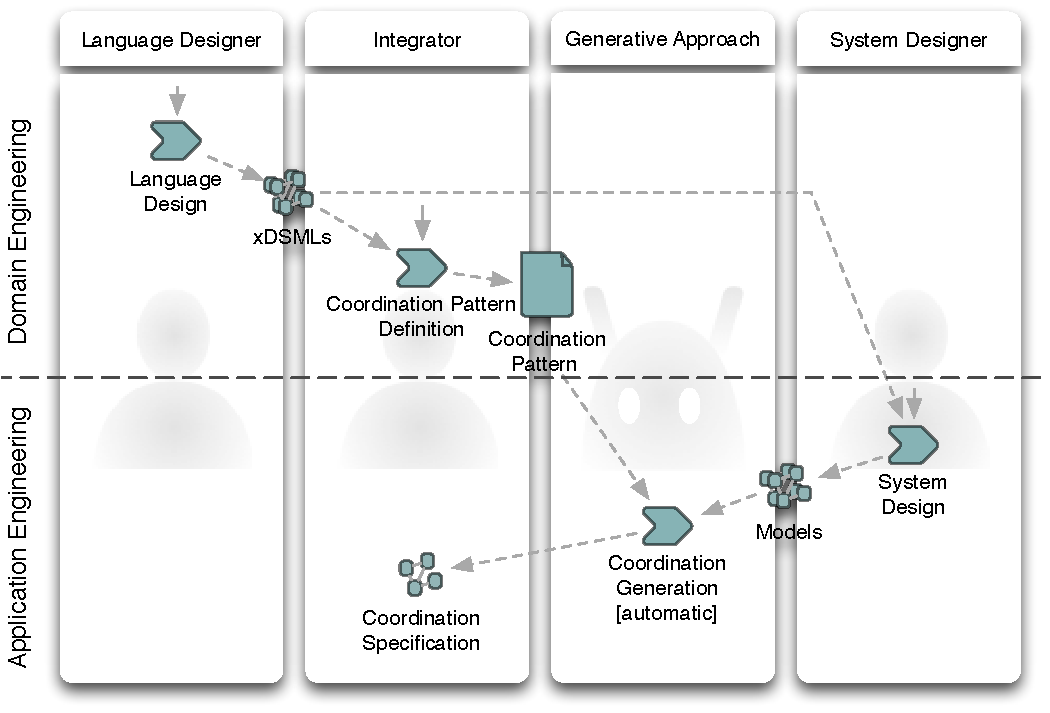
\includegraphics[width=.6\textwidth]{bcool/figs/process}
		\caption{The proposed workflow}
		\label{fig:proposedworkflow}
	\end{center}
\end{figure}

%The running example helps us to illustrate the different tasks in the development of heterogeneous systems:
%	\begin{enumerate}
%		\item Designing of the languages.
%		\item Integration of the languages. 
%		\item Building of the models. 
%		\item Coordination of the models. 
%	\end{enumerate}
%In this context, \bcool deal with the task number two and four. 